%Het eerste hoofdstuk van je thesis.
\chapter{Literatuurstudie}
De literatuurstudie schetst een beeld van de sateliet constellaties die gebruikt worden. Deze worden besproken in \ref{LGNS}. Eens we de verschillende types van satelieten kennen, besrpeken we de manier waarop ze met elkaar communiceren in sectie \ref{LCom}.

\section{GNSS}
\label{LGNS}
GNSS ofwel Global Navigation Satellite System, is een sateliet systeem met een wereldwijde dekking. GNSS is een standaard term gebruikt om systemen te beschrijven die positie en navigatie oplossingen bieden. Het werd voornamelijk ontwikkeld voor de luchtvaart en ruimtevaart industrie en militaire doeleinden. Tegenwoordig worden deze technologie\"en ook in andere toepassingen gebruikt. GNSS vraagt samenwerking tussen verschillende publieke en private organisaties \cite{LBibGNSS3}.  Dit systeem is opgebouwd uit verschillende subsystemen die verder in deze tekst bepsroken worden. Namelijk: GPS besproken in sectie \ref{LGPS}, In sectie \ref{LGLO} bespreken we GLONASS, Galileo wordt besproken in sectie \ref{LGal} en BeidDou komt al laatste aan bod in sectie \ref{LBeD}. Het IGS, International GNSS Service staat in voor de aflevering van de hoogste kwaltieit GNSS data en producten \cite{LBibGNSS}. Elke satelliet is een project op zichzelf. Hierdoor is het moeilijk om een gestandaardiseerde productie ketting te creëren \cite{LBibGNSS3}.

\subsection{GPS}
\label{LGPS} 
GPS staat voor Global Positioning System. Dit is het satelieten gebaseerde positie systeem dat bij ons het bekendste is. Het is ontwikkeld in Amerika \cite{LBibGNSS}\cite{LBibGNSS3}. het is \'e\'en van de langst gebruikte systemen binnen GNSS en draait momenteel op volledige capaciteit \cite{LBibGNSS4}. Voor de gebruikers is kost van de data een hoge bezorgdheid. Daarom is het belangrijk om de kosten van de operaties te verkleinen. GPS moet toegankelijk zijn voor meerdere clients. De gebruikerstoegang gebeurt voornamelijk door mobiele toestellen die verbindig maken via het internet \cite{LBibGPS}. De constellatie van GPS bestaat uit 32 satellieten en heeft zijn volledgie functionele capaciteit bereikt (FOC), het systeem wordt geleidelijk aan gemoderniseerd \cite{LBibGNSS4}.

\subsubsection{Manieren om posities te bepalen}
\paragraph{Differential GPS Corrections}
Differential GPS Corrections ook weel DGPS genoemd, worden gebruikt om nauwkeurig posities  te bepalen. Er worden minimaal twee GPS ontvangers gebruikt. Van \'e\'en van deze ontvangers moet de preciese postie gekend zijn. De positie van het andere station kan dan geschat worden door een vergelijking van de co\"ordinaten van de twee stations. Dit is een populaire manier om sateliet en klok fouten te elimineren. Een nadeel van deze techniek is dat de observaties van beide stations simultaan moeten gebeuren \cite{LBibGNSS2}. 

\paragraph{Precise Point Positioning}
of PPP is een techniek die werkt met \'e\'en ontvanger en is zeer effeci\"ent. \cite{LBibGNSS4}

\subsection{GLONASS}
\label{LGLO}
GLONASS is \'e\'en van de langst gebruikte systemen binnen GNSS. Het is ontwikkeld door Rusland \cite{LBibGLONASS2}. GLONASS is een afkorting, het staat voor GLObal NAvigation Satelite System \cite{LBibBeiDou}. Het systeem is volledig gerevialiseerd en is volledig operationeel. De constellatie is opgebouwd uit 24 satelieten. \cite{LBibGNSS4}. Deze satelliten zijn geplaatst in drie orbitale vlakken met een onderlinge afstand van 120 graden\cite{LBibGLONASS2}. Het systeem heeft zijn FOC bereikt in januari 1996. \cite{LBibGLONASS}.Het GLONASS systeem is opgebouwd uit vier elementen:
\begin{itemize}
	\item Orbitale constellatie van GLONASS satellieten
	\item Controle segment op de grond
	\item Racket/ruimte complex
	\item Gebruikers
\end{itemize} \cite{LBibGLONASS2} Het systeem wordt continu gemoderniseerd \cite{LBibGNSS4}. GLONASS-M satellieten vormen een tweede genereatie van satellieten die gebruikt worden. Deze tweede generatie heeft volgende voordelen:
\begin{itemize}
	\item Langere gegarandeerde levenstijd (zeven jaar in plaats van drie)
	\item Maakt gebruik van L2 signalen
	\item Stabielere klok
	\item Extra beschikbare navigatie data (zoals betere integritetiscontrole, informatie over absolute tijd beschikbaarheid van de satelliet nummer)
	\item inter-satellite radio link
	\item Betere zonnenpanelen postionering
	\item Lager niveau van onvoorspelde versnellingen
\end{itemize}
Door deze tweede generatie GLNOASS-M satellieten zijn er nieuwe mogelijkheden voor satelliet navigatie. GLONASS is een betrouwbaar systeem, voornamelijk voor Real-Time Kinematic (RTK) mode in omgevingen met slechte zichtbaarheid \cite{LBibGLONASS}. Voor de werking van het navigatie satelliet systeem is het belangrijk dat alle plrocessen die plaats vinden tijdens de werking gesynchroniseerd zijn. GLONASS-K satelieten vormen de derde generatie. De grootste veranderingen ten opzichte van GLONASS M zijn:
\begin{itemize}
	\item Het gebruik van een derde frequentie om betrouwbarheid en nauwkeurigheid voor gebruikersnavigatie te vergroten.
	\item De levensduur van de satelliet is vergroot tot 10 jaar
	\item Het gewicht van de satelliet is gehalveerd
\end{itemize}\cite{LBibGLONASS2}.

\subsection{Galileo}
\label{LGal}
Galileo is het Europees systeem \cite{LBibGNSS3}\cite{LBibGNSS4}. Het doel van Galileo is het aanbieden van een flexibelere en nauwkeurige postionerings service \cite{LBibGNSS4}. De architectuur van Galileo specificeert een globaal integriteits concept. Dit wilt zeggen dat de naugeruigheid en de integriteit van de werking altijd wereldwijd bereikt moet worden en binnen de drempelwaarden moet blijven \cite{LBibGalileo}.  De volledige constellatie zal bestaan uit 30 satelieten in drie orbitale vlakken. Het systeem is momenteel nog onder contructie \cite{LBibGNSS4}.  Het Galileo systeem voorziet verschillende gebruikersdiensten. E\'en van deze diensten is de Safety of Life service, dit is een groot voordeel van Galileo on vergelijking met GPS. In geval van een systeem fout moet de gebruiker binnen de zes seconden gewaarschuwd worden \cite{LBibGalileo}. 

\subsection{BeiDou}
\label{LBeD}
BeiDou is het satilieten systeem binnen GNSS dat ontwikkeld is in China. Het systeem wordt vaak aangeduid met de afkorting BDS \cite{LBibBeiDou} Het voorziet PNT (Postioning, Naviagtion and Timing) services in de Aziatisch-Pacifische regio. De volledige constellatie telt 35 satelieten. Het zal volledig zijn tegen het einde van 2020 \cite{LBibGNSS4}. Momenteel is BDS beshikbaar voor regionale diensten. Eveneens in 2020 zullen BDS signalen beschikbaar worden voor wereldwijde gebruikers. Ondertussen worden er steeds meer stations uitgebreid met BDS ontvangers voor hoog-precisie GNSS toepassingen \cite{LBibBeiDou}.

\subsection{Besluit}
Eens de vier systemen volledig ingezet zijn, zijn er meer dan 100 satelieten beschikbaar voor nauwkeurige PNT toepassingen. Door het opkomen van de twee nieuwere systemen Galileo \ref{LGal} en BeiDou \ref{LBeD} en de het voortdurend moderniseren van GPS \ref{LGPS} en GLONASS \ref{LGLO} is de wereld van sateliet navigatie onderheving aan veranderingen. \cite{LBibGNSS4}.Momenteel loopt er een Mutli-GNSS expirment (MGEX) dat data verzamelt van GPS?GLONASS, Galileo en BeiDou. De samenvoeging van multi-GNSS vergroot het aantal satellieten en bijgevolg wordt de geometrische observatie geoptimaliseerd \cite{LBibGNSS5}. De multiple-GNSS observaties met meerdere frequenties voorzien de onderzoekers van meerdere kansen om de Aardse ionosferische variaties en gedragingen te onderzoeken. GNSS observaties kunnen gebruikt worden om ionosferische traagheids correcties en gerelateerd atenschappelijk onderzoek \cite{LBibBeiDou}.

\section{Communicatie}
\label{LCom}
\subsection{EUREF Permanent Netwerk}
Het EUREF Permanent Network wordt ook wel EPN genoemd. Het netwerk is opgebouwd uit 190 permanenten GPS stations waarvan er 29 ook GLONASS satellieten volgend. Het primaire doel van EPN is het Euroean Terrestrial Reference Systems (ETRS) onderhouden. \cite{LBibEPN}.

\subsection{RTCM}
RTCM staat voor Radio Technical Commission for Maritime Services \cite{LBibGLONASS}.

\subsection{NTRIP}
\label{LNTR}
Networked Transport of RTCM via Internet Protocol of kortweg NTRIP. Men maakt gebruik vant internet om de realtime GNSS data uit te wisselen en te verzamelen. NTRIP is een HTTP(Hypertext Transfer Protocol) stateless applicatie level protocol om GNSS data te streamen over het internet. De nodige brandbreedte hiervoor is niet groot in vergelijking met bijvoorbeeld Internet Radio\cite{LBibNTRIP}. Het is gebaseert op software die oorspronkelijk bedoelt was voor MP3 media speler formaten. Dit blijk wel aangepast te zijn voor GNSS stromen met data snelheden toosen 0.5 en 5 kbit/s. \cite{LBibGPS}. Een ander voordeel is dat tegenwoordig op veel plaatsen internet verbinding voorzien is \cite{LBibNTRIP}

\subsubsection{opbouw van NTRIP software}
\label{LONS}
NTRIP wordt ge\"implemeneteerd in drie systeem software componenten. Nameijk Ntrip clients, NtripServers en NtripCasters. De NtripCaster is het HTTP server programma terwijl NTRIPClients en NTRIPServers reageren zoals HTTP clients\cite{LBibNTRIP}. NTRIPServers gaat datastromen vervoeren. NTRIPCasters gaan de administratie tussen clients en datastromen afhandelen \cite{LBibGPS}. NTRIPCasters is een stream-spliteser en broadcaster component, momenteel zijn er acht NTRIPCasters in Europa. NTripClients gaan data ontvangen van de gewenste bronnen via de NTRIPCaster. NTRIPServers gaan de data van \'e\'en of meerdere bronnen verzenden in NTRIP formaat. Als laatste hebben we ook nog NTRPSorurces, deze genereren DPGS datastreams op een specifieke locatie. \cite{LBibNTRIP} In figuur \ref{imgNTRIP} staat een overzicht van de opbouw van het NTRIP streaming systeem.

\begin{figure}[hpb]
	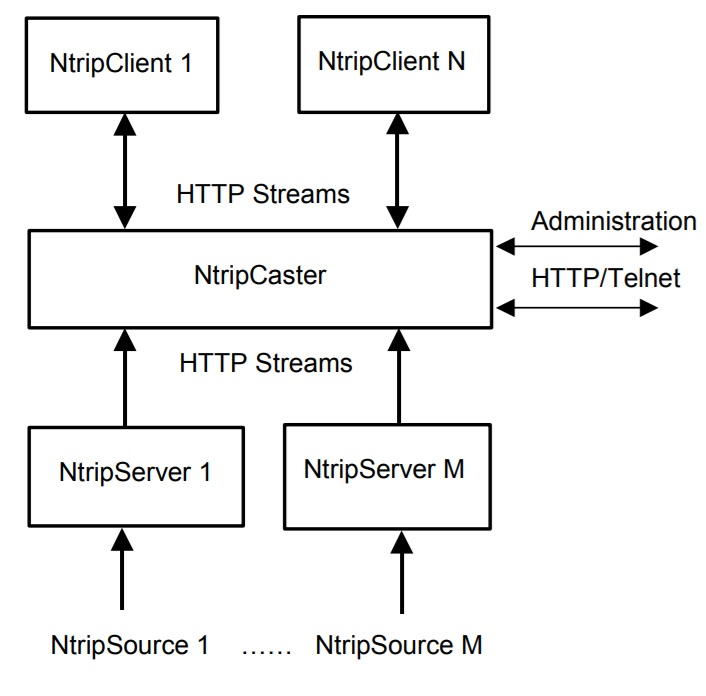
\includegraphics[scale=0.65]{NTRIP.jpg}
	\caption{NTRIP streaming systeem}
	\cite{LBibNTRIP}
	\label{imgNTRIP}
\end{figure} 
 



